\documentclass[a4paper,12pt]{article}
\usepackage{a4wide}
\usepackage{tikz}
\usetikzlibrary{calc}
\usepackage{hyperref}
\usepackage{color}
\usepackage{pdflscape}
\usepackage{bytefield}

\newlength{\maxheight}
\setlength{\maxheight}{\heightof{W}}
\newcommand{\baselinealign}[1]{%
	\centering
	\raisebox{0pt}[\maxheight][0pt]{#1}%
}

\newcommand\Tstrut{\rule{0pt}{2.6ex}}       % "top" strut

\definecolor{grau}{gray}{.5}  

\begin{document}
\pagestyle{empty}
\setlength{\parindent}{0em} 
\section*{Single Cycle Control Unit}

Your task is to program the behavior of an entity called ``SC\_CU". This entity is declared in the attached file ``SC\_CU.vhdl" and has the following properties:
\begin{itemize}
\item Input:  Opcode with type std\_logic\_vector of length 6
\item Input:  Funct with type std\_logic\_vector of length 6
\item Input:  Zero with type std\_logic
\item Output: ALUControl with type std\_logic\_vector of length 3
\item Output: Control signals RegDst, Branch, Jump, MemRead, MemtoReg, MemWrite, ALUSrc and RegWrite all with type std\_logic
\end{itemize}

\begin{center}
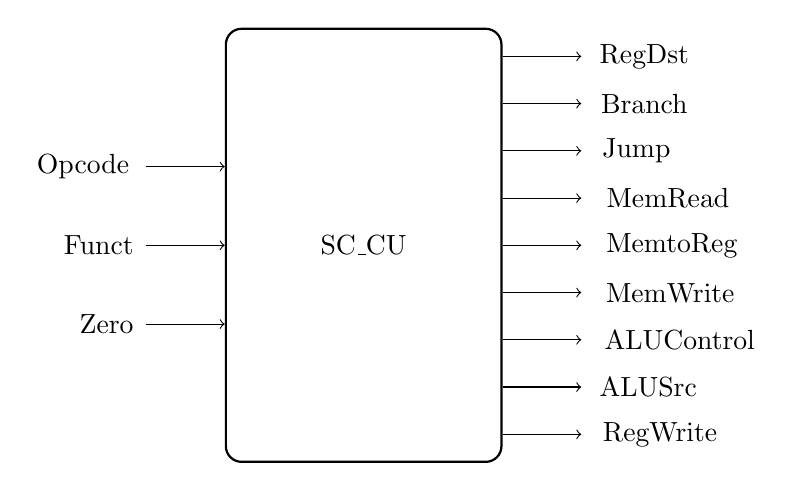
\begin{tikzpicture}
\draw node [draw,rectangle, minimum height=55mm, minimum width=35mm,rounded corners=2mm,thick](entity){};

\draw[->] ($ (entity.west)+(-10mm,10mm)$) -- ($ (entity.west) + (0mm,10mm)$);
\draw node at ($ (entity.west)-(18mm,-10mm)$){Opcode};

\draw[->] ($ (entity.west)-(10mm,0mm)$) -- ($ (entity.west) - (0mm,0mm)$);
\draw node at ($ (entity.west)-(16mm,0mm)$){Funct};

\draw[->] ($ (entity.west)-(10mm,10mm)$) -- ($ (entity.west) - (0mm,10mm)$);
\draw node at ($ (entity.west)-(15mm,10mm)$){Zero};


\draw[->] ($ (entity.east) + (0mm,24mm)$) -- ($ (entity.east) + (10mm,24mm)$);
\draw node at ($ (entity.east) + (18mm,24mm)$){RegDst};

\draw[->] ($ (entity.east) + (0mm,18mm)$) -- ($ (entity.east) + (10mm,18mm)$);
\draw node at ($ (entity.east) + (18mm,18mm)$){Branch};

\draw[->] ($ (entity.east) + (0mm,12mm)$) -- ($ (entity.east) + (10mm,12mm)$);
\draw node at ($ (entity.east) + (17mm,12mm)$){Jump};

\draw[->] ($ (entity.east) + (0mm,6mm)$) -- ($ (entity.east) + (10mm,6mm)$);
\draw node at ($ (entity.east) + (21mm,6mm)$){MemRead};

\draw[->] ($ (entity.east) + (0mm,0mm)$) -- ($ (entity.east) + (10mm,0mm)$);
\draw node at ($ (entity.east) + (21.5mm,0mm)$){MemtoReg};

\draw[->] ($ (entity.east) + (0mm,-6mm)$) -- ($ (entity.east) + (10mm,-6mm)$);
\draw node at ($ (entity.east) + (21.3mm,-6mm)$){MemWrite};

\draw[->] ($ (entity.east) + (0mm,-12mm)$) -- ($ (entity.east) + (10mm,-12mm)$);
\draw node at ($ (entity.east) + (22.5mm,-12mm)$){ALUControl};

\draw[->] ($ (entity.east) + (0mm,-18mm)$) -- ($ (entity.east) + (10mm,-18mm)$);
\draw node at ($ (entity.east) + (18.5mm,-18mm)$){ALUSrc};

\draw[->] ($ (entity.east) + (0mm,-24mm)$) -- ($ (entity.east) + (10mm,-24mm)$);
\draw node at ($ (entity.east) + (20mm,-24mm)$){RegWrite};

\draw node at ($ (entity) - (0,0mm)$){SC\_CU};

\end{tikzpicture}
\end{center}

Do not change the file ``SC\_CU.vhdl".\\


You will have to implement the following types of instructions:
%%SELECTED_INSTRUCTIONS_TYPE

The ``SC\_CU" entity shall control the single cycle processor depicted in Figure~1 to perform the following instructions:

\begin{table}[h!]
\centering
    \begin{tabular}{|c|c|c|c|c|} \hline \Tstrut
		instruction & opcode  & funct	& zero & type   \\ \hline \Tstrut
		%%SELECTED_INSTRUCTIONS
    \hline
    \end{tabular}
\end{table}

%%SELECTED_INSTRUCTIONS_TEXT

\begin{table}[h!]
\centering
    \begin{tabular}{|c|c|} \hline \Tstrut
		ALUControl & Function   \\ \hline \Tstrut
		%%SELECTED_ALUCONTROLS
    \hline
    \end{tabular}
    \caption{ALUControls}
    \label{tab:ALUControls}  
\end{table}

Consider which actions each part of the processor in Figure~1 has to take to fulfill the functions of the operations and set the control signals accordingly. This behavior has to be programmed in the attached file ``SC\_CU\_beh.vhdl".\\

To turn in your solution write an email to %%SUBMISSIONEMAIL with Subject ``Result Task %%TASKNR" and attach your file ``SC\_CU\_beh.vhdl".

\vspace{0.7cm}
Good Luck and May the Force be with you.

\begin{landscape}
\begin{figure}[!h]
\vspace{-0.5cm}
\hspace{-1.8cm}
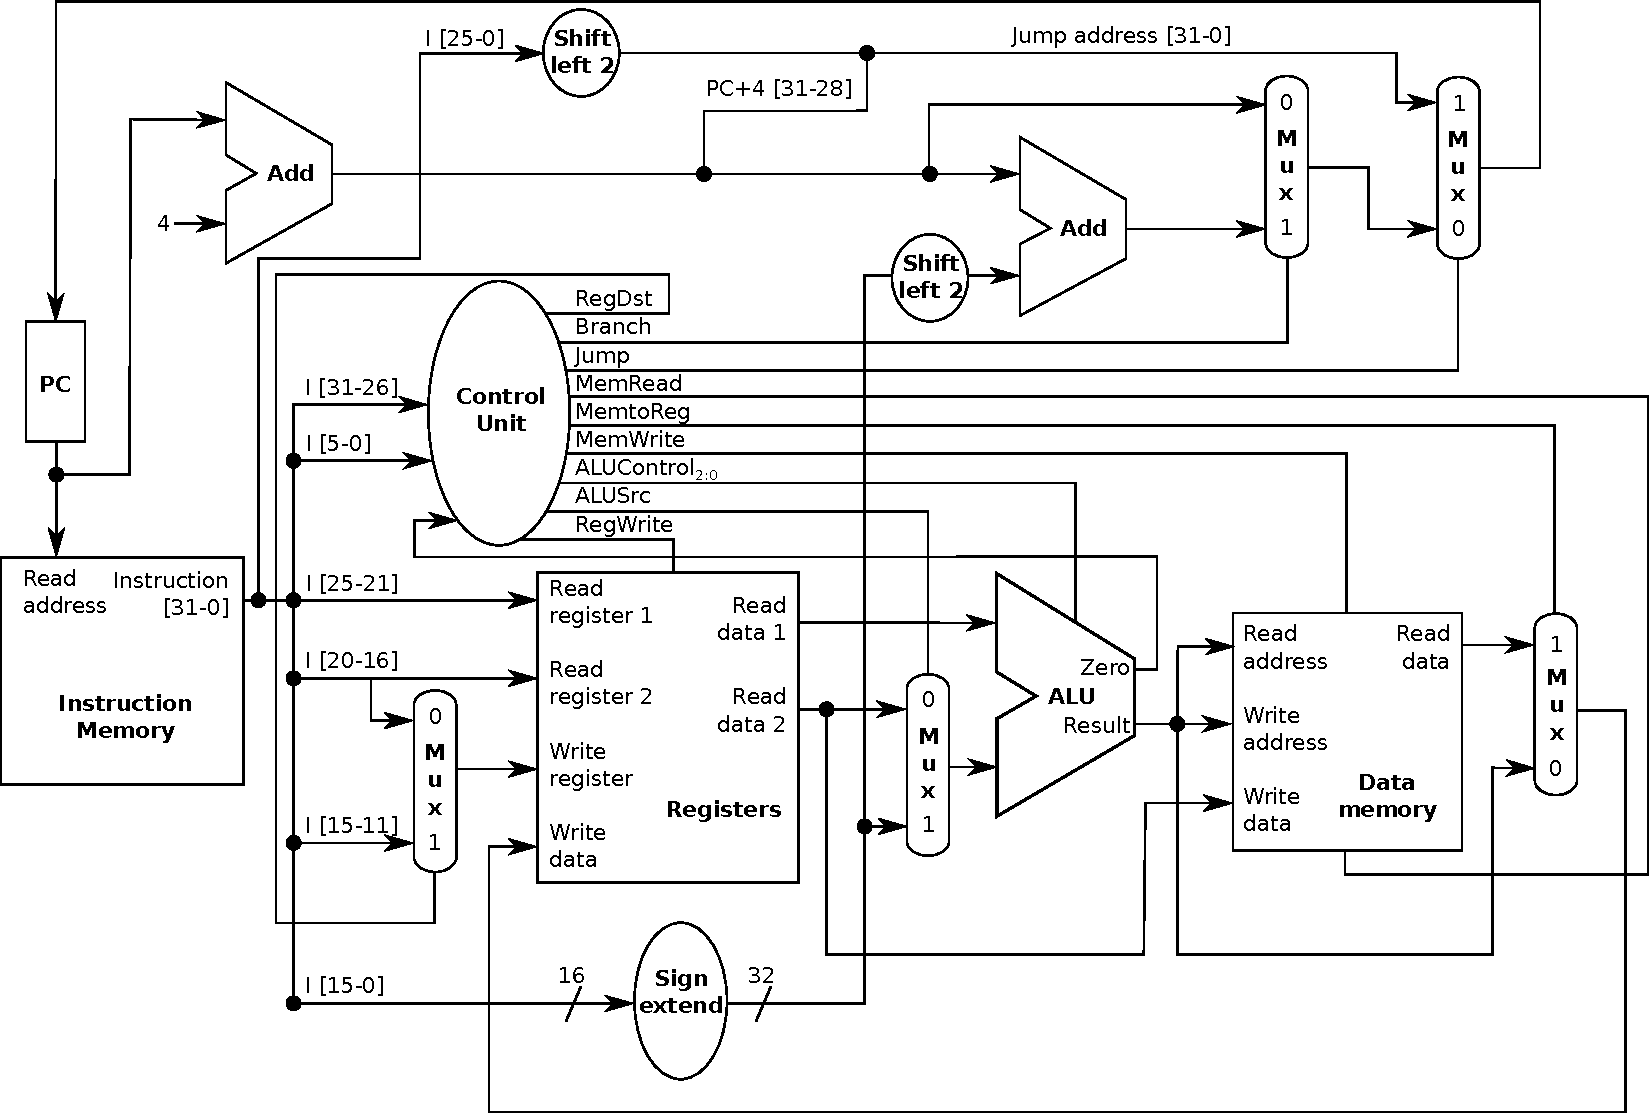
\includegraphics[width=25.5cm]{Single_Cycle_Processor_V_3_0}
\caption{Single cycle processor}
\label{fig:SingleCycleProcessor}
\end{figure}
\end{landscape}


\end{document}